\section{Höhenprofil}

\begin{figure}[h]
    \centering
    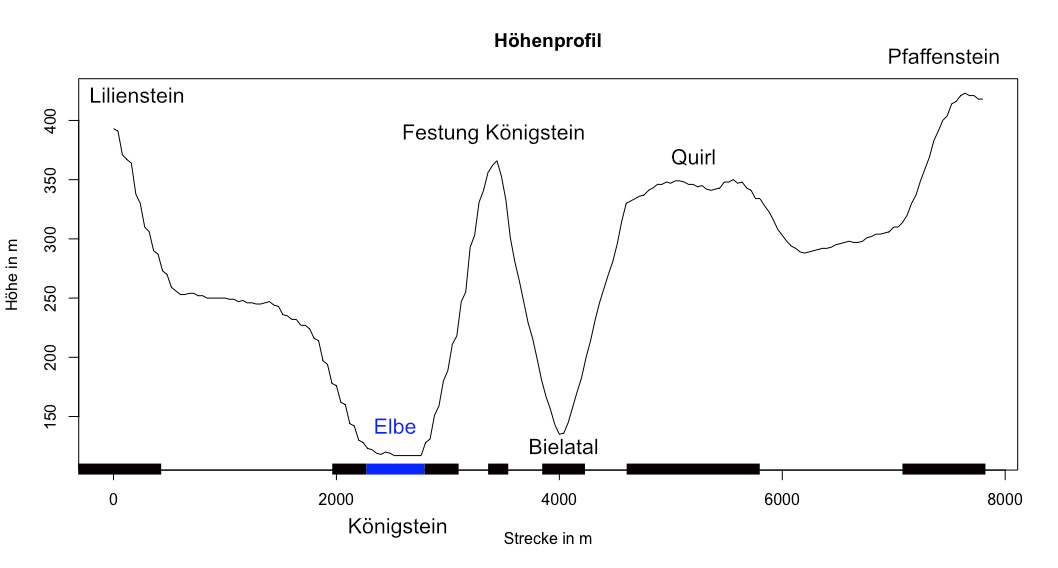
\includegraphics[scale = 0.40]{Abbildungen/Hoehenprofil.jpg}
    \caption{Höhenprofil anhand TK von A über B und C nach D. Auf Grundlage von SRTM Daten}
    \label{fig:abb2}
\end{figure}

Im folgenden wird das erstellte Höhenprofil aus Abbildung \ref{fig:abb2} mit der Strecke zwischen A (Lilienstein) über B (Königstein) und C(Quirl) bis D (Pfaffenstein) beschreiben. 

Ein Höhenprofil 

Die Strecke befindet sich in der Region um die Stadt Königstein. Die Gesamtstrecke beträgt eine Länge von ungefähr 8 km. Der größte Höhenunterschied zwischen dem Gipfel des Pfaffensteins auf 423 Höhenmetern und dem tiefsten Punkt der Elbe auf 117 Höhenmetern liegt bei 300 Höhenmetern. Weitere wichtige Hoch- und Tiefpunkte sind der Lilienstein bei 390 Höhenmetern, der Königstein bei 366 Höhenmetern, das Bielatal bei 135 Höhenmetern und der Quirl bei 330 Höhenmetern. 

Der erste Abschnitt von A (Lilienstein) zu B (Königstein) beginnt auf 390 Höhenmetern. Der Streckenverlauf beginnt mit einem steilen Hang, der sich über 500m Luftlinie erstreckt und mit 140m Differenz auf 250 Höhenmetern absinkt. Auf der selben Höhe folgt eine flachere Plateau Ebene, die mit Feldern bewirtschaftet ist. Diese erstreckt sich über 900m Luftlinie. Der Abstieg geht mit einem leicht steilen Hang für 350m Luftlinie weiter. Dabei sinkt die Höhe nur um 50m auf 200 Höhenmeter. Diese Region ist Bebaut. Es geht mit einem steileren Teil weiter. Dieser sinkt über 200m Luftlinie um 80m auf 117 Höhenmetern, den tiefsten Teil des Höhenprofils ab. Hier befindet sich der Fluss die Elbe, in Abbildung \ref{fig:abb2} Blau markiert. Dieser erstreckt sich über 300m Luftlinie, was nicht der tatsächlichen Breite entspricht, da der Fluss anhand der Strecke nicht durch den kürzesten Weg gequert wird.  Der Abstieg ist nun vorbei. Weiter geht es mit einem steilen Hang um die 200m Luftlinie, der auf 200 Höhenmetern aufsteigt. Hier befindet sich Bebauung der Stadt Königstein. Danach geht der Hang ohne Bebauung weiter ung steigt auf 366 Höhenmetern bis zur Festung Königstein auf, welche sich auf dem Gipfel des Berges befindet. Insgesamt beträgt der Abschnitt A bis B 3350m Luftlinie und ist damit der längste der drei Abschnitte.

Der zweite Abschnitt von B (Königstein) zu C (Quirl) beginnt wieder mit einem steilen Abstieg von der Festung Königstein auf 366 Höhenmetern bis in das Bielatal auf 135 Höhenmetern. Dieser Abstieg erstreckt sich über 650m Luftlinie. Im Bielatal befindet sich weitere Bebauung der Stadt Königstein. Anliegend geht es wieder über 800m Luftlinie Bergauf bis auf 330 Höhenmeter bis zum Quirl. Insgesamt beträgt der Abschnitt B bis C 1450m Luftlinie und ist damit der kürzeste der drei Abschnitte

Der letzte Abschnitt von C (Quirl) bis D (Pfaffenstein) beginnt mit dem Quirl selbst der sich über 1200m Luftlinie in einer art Plateau erstreckt. Hierbei steigen und sinken die Höhenmeter um rund 20m. Nach dem Plateau geht es für 300m Luftlinie Bergabwärts auf 290m. Ab da geht es für 900m Luftlinie leicht bergauf auf 320m. Der Anstieg ist so flach das auch hier mit Feldern bewirtschaftet wird. Der letzte Teil der Strecke ist wieder ein steiler anstieg zum Höchsten Punkt der Strecke, dem Gipfel des Pfaffensteins, auf einer Höhe von 423m. Dieser anstieg erstreckt sich über 600m Luftlinie und legt dabei 100 Höhenmeter zu. Insgesamt beträgt der Abschnitt C bis D 3000m Luftlinie.